\documentclass[]{article}

\usepackage[numbers]{natbib}

%opening
\usepackage{float}
\usepackage[hidelinks]{hyperref}
\usepackage{scrextend}
\usepackage[utf8]{inputenc}
\usepackage{graphicx}
\usepackage{listings}
\usepackage{color}
\usepackage{tocloft}
%\renewcommand{\cftpartleader}{\cftdotfill{\cftdotsep}} % for parts
%\renewcommand{\cftchapleader}{\cftdotfill{\cftdotsep}} % for chapters
\renewcommand{\cftsecleader}{\cftdotfill{\cftdotsep}} % for sections, if you really want! (It is default in report and book class (So you may not need it).
\setlength{\parskip}{16pt}

\title{Project Assignment Part II:\@ Simulation of a base scenario }

\author{Jef Jacobs \\ Toon Eeraerts \\ Wout Deleu}
\date{Semester 2}

\begin{document}
\setlength{\parindent}{0pt} \maketitle \tableofcontents \newpage %geen indent bij nieuwe paragraaf

\section{Introduction}
For this assignment, a base scenario of the `Yard storage assignment problem'
was implemented and simulated. During this report, the basics design choices
will be discussed, as well as the results of the simulation.

The basic technology used is Python. The code is written as dynamic as
possible, using global variables and booleans to variate parameters and the
overall flow of the simulation. The simulation is based on a discrete event
simulation, with the possibility of online simulation.

To refresh the environment in brief, the goal is to simulate a yard, in which
containergroups\footnote{Containers arrive only in group. Containers are (for
	now) not looked at individually. This means they can't be split up, they are
	stored in the same place, they enter and leave the yard at the same time.} come
and go. They can arrive from vessels or from trucks and trains. The goal is to
simulate the storage situations in the yard, as a result of the in and out
flow.

\section{Simulation parameters}
The first and maybe most primary parameter to know is the amount of simulations
that needs to be run to get significant results. This can be calculated by the
following formula: $$ JEF HEEFT EEN KLEINE PENIS $$

\subsection{Generation of parameters}
In order to emulate the basic behavior of the yard, there needs to be a stream
of containergroups, with their own properties. To perform an online simulation,
this stream needs to be generated on the fly. In the prior assignment, a study
was held to figure out distributions, which will be used to generate the
necessary information regarding the containergroups. This is necessary to
generate the input to feed the simulation.

The generation of the groups happens at random times, which are calculated
using the arrival time of the previous group, and a random interval time. This
interval time is being generated using an exponential function based upon the
input data analysis of Nick De Bruyckere, Enrique Miron and Dries Van de Velde
(Figure \ref{fig: inter arrival time analysis}).
\begin{figure}[!tbp]
	\centering
	\begin{minipage}[b]{0.40\textwidth}
		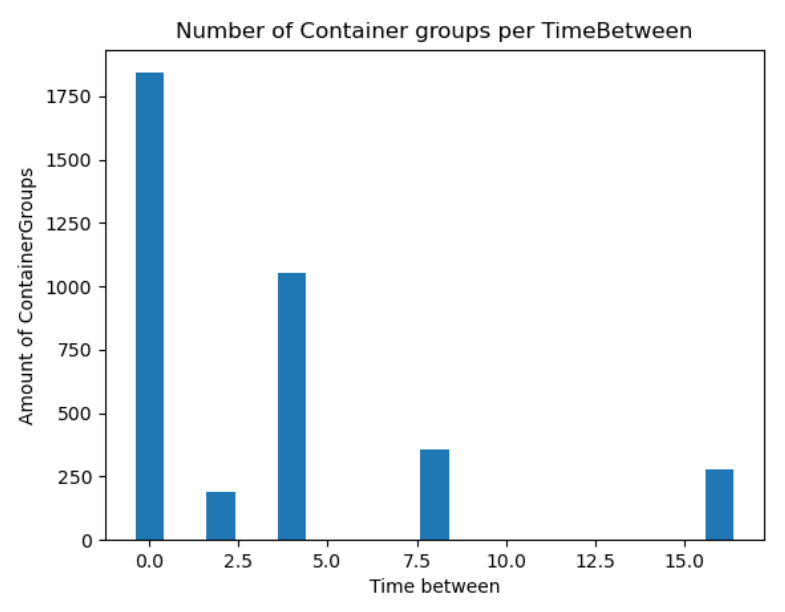
\includegraphics[width=\textwidth]{Afbeeldingen/inter_arrival_times_hist.png}
		\caption{Inter arrival time in prior analysis}
		\label{fig: inter arrival time analysis}
	\end{minipage}
	\hfill
	\begin{minipage}[b]{0.44\textwidth}
		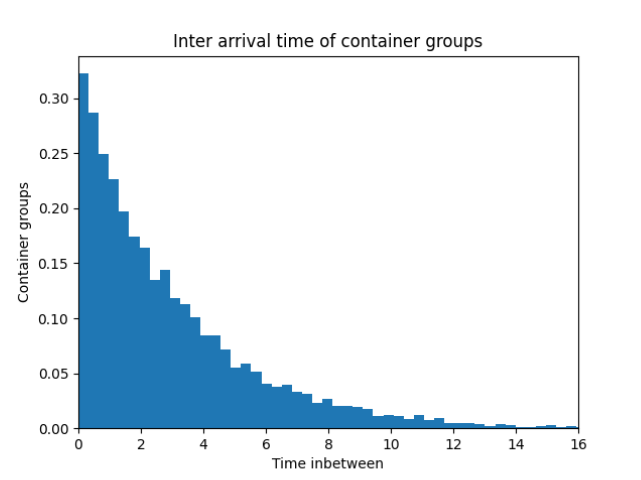
\includegraphics[width=\textwidth]{Afbeeldingen/inter_arrival_time_sample.png}
		\caption{Inter arrival time sample distribution used in the simulation}
	\end{minipage}
\end{figure}

When the arrival time of a batch of containers is determined, some properties
of that container group needs to be generated. The properties are:
\begin{itemize}
	\item The type of containers
	\item The number of containers in the group
	\item The service time needed
	\item The arrival position of the group
	\item The departure position of the group
	\item The flow type (which can be import or export)
\end{itemize}

The type of containers is also based upon the input analysis of Nick De
Bruyckere, Enrique Miron and Dries Van de Velde represented in Figure \ref{fig:
	container type analysis}. Normal containers and reefer container occur
respectively 69\% and 31\% of the times.
\begin{figure}
	\centering
	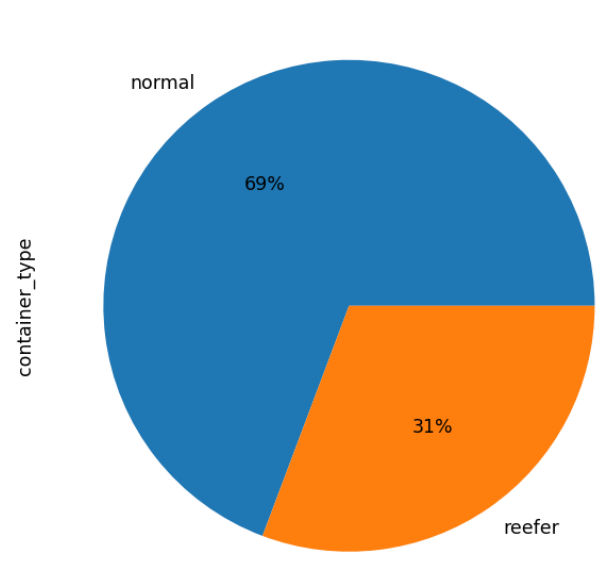
\includegraphics[width=0.5\textwidth]{Afbeeldingen/container_type.png}
	\caption{Container type analysis}
	\label{fig: container type analysis}
\end{figure}

Each group has a certain amount of containers in them. This is chosen based
upon our own analysis of the input data. The distribution is represented by a
steep exponential distribution which is never lower than 1. (Figure: \ref{fig:
	container group size sample})
\begin{figure}[!tbp]
	\centering
	\begin{minipage}[b]{0.45\textwidth}
		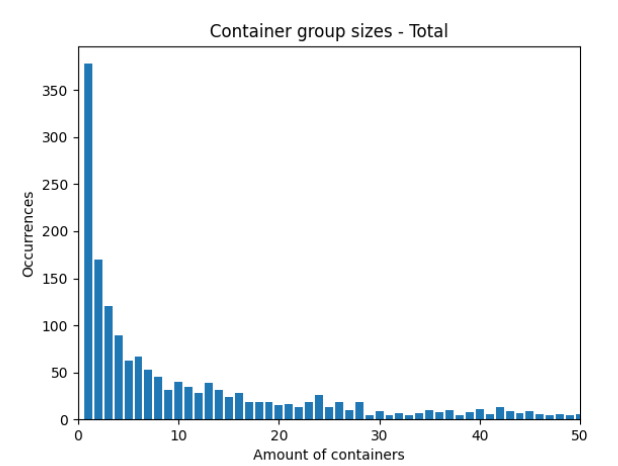
\includegraphics[width=\textwidth]{Afbeeldingen/container_group_sizes.png}
		\caption{container group size analysis}
	\end{minipage}
	\hfill
	\begin{minipage}[b]{0.44\textwidth}
		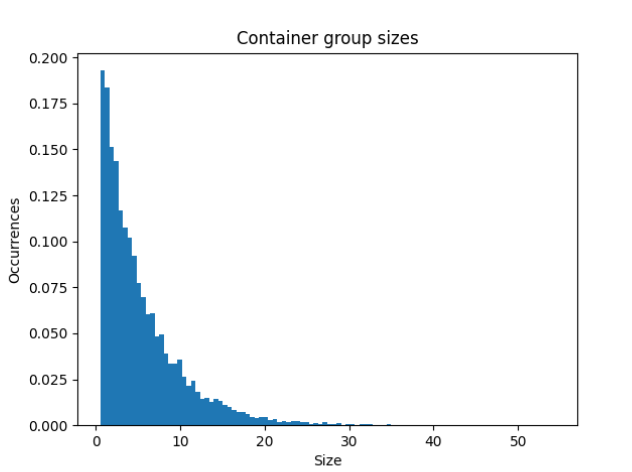
\includegraphics[width=\textwidth]{Afbeeldingen/container_group_size_sample.png}
		\caption{Cointainer group size sample distribution}
		\label{fig: container group size sample}
	\end{minipage}
\end{figure}

Each instance has a service time, which is the time containers needs to stay in
the yard before further actions are taken. This factor is directly dependent on
the flow type. If it is import or export, the service time is by default 48
hours. But if it is stated as a transhipment (which is technically a subtype of
export), than it can vary between 0 and 166 hours. Ths is based upon our own
analysis of the input data whic shows a uniform distribution between 0 and 166
hours (Figure \ref{fig: service time analysis}). For this reason, the service
time sample always takes a random number between these two values.
\begin{figure}
	\centering
	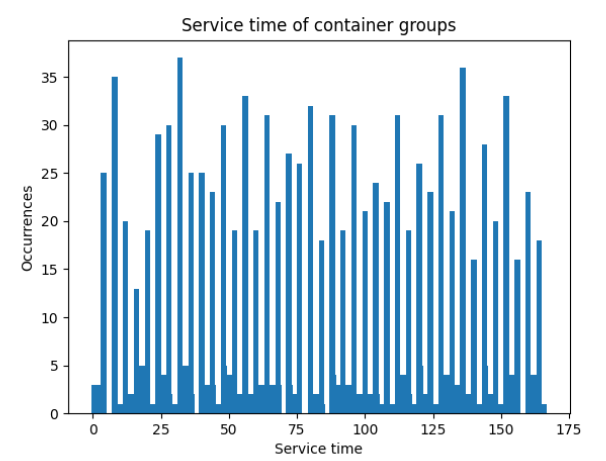
\includegraphics[width=0.5\textwidth]{Afbeeldingen/service time analysis.png}
	\caption{Service time analysis}
	\label{fig: service time analysis}
\end{figure}

The arrival and departing position of vessels and trucks is randomly selected
out of the available locations.

\subsection{Resulting values}
Each simulation run will store different characteristics which, will be used to
evaluate the performance of the simulation. The most important characteristics
are: \begin{itemize}
	\item Amount of rejected containers and container groups (total and for each type
	      individually)
	\item The total and average travel distance
	\item Per YardBlock:
	      \begin{itemize}
		      \item The maximal occupancy at any given time
		      \item The maximal occupancy per day (\textbf{= average occupancy per day})
	      \end{itemize}
	\item Average daily occupancy over all containers: The average occupancy per day over
	      all the YardBlocks \[\forall i \in days: \frac{\sum_{(x \in YardBlocks)}
			      \overline{Occupancy_{i,x}}}{\#YardBlocks}\]
\end{itemize}

After seeing the first tests, i t was clear that with 159 Yardblocks in total,
it is not the most useful thing to list the individual occupancy for every
block, and include this in this rather short report. But to give an idea of
this data, some basic statistics are given over the data: \begin{itemize}
	\item The amount of YardBlocks which are close to being full (90\% average
	      occupancy\footnote{\label{margin} Because the simulation is run many times, the
		      averages of 100\% for example are hard to reach, thats why a small margin has
		      been taken into account.})
	\item The amount of YardBlocks which are never used (5\% average
	      occupancy\footref{margin})
\end{itemize}

\section{Results}

\subsection{Basic scenario}
The basic scenario that is discussed in this report describes a decision rule
which stores every containergroup that arrives, if there is space in the yard.
If there is no space, the container is rejected. This will be referred to as
\textit{FIFO (First In First Out)}. This apply's to arrival of containers, and
wether or not they are kept in the yard. FIFO says that the first container
that arrives, has a priority over the ones which arrive after the first one. If
there is no space for an arriving containergroup, it will be rejected. While
the next containergroup arrives, the check for space will happen again, and so
on.

Two different approaches to block assignment are implemented. The block
assignment rule has affect on which block is chosen to store a containergroup.
The two different situations studied here are \textit{arrival based} and
\textit{departure based}. Arrival based and departure based both are both based
on the minimal distance between 2 points. The yard block chosen is the closest
block to the arrival point, in case of arrival based, or closest to the
departure point, in case of departure based.

The 2 different approaches give somewhat similar results. The main difference
is in the travel distance. This is significantly higher with departure based
approach. This could be explained by the fact that groups leave the yard on
more similar positions, than they arrive, which could lead to containers being
stored somewhat further from there optimal point. This is a rather unlikely
scenario, because individual blocks are (almost) never close to full. It is
consequently unlikely containergroups would be stored somewhere else than it's
optimal position. Another and more likely explanation is that the temporary
storage of containers on the yard could, when searching for the closest block
to the departure point, is further from the optimal route than when searching
for the closest block to the arrival point. This can maybe a vague description,
but on Figure \ref{fig:closest} could clarify this. Point A could be an arrival
point, point D a departure point. C1 is the yardblock closest to the arrival
point, and C2 to the departure point. The shortest path from A to B is the
straight line. We can see that C2 is further from the optimal path than C1.
\begin{figure}
	\centering
	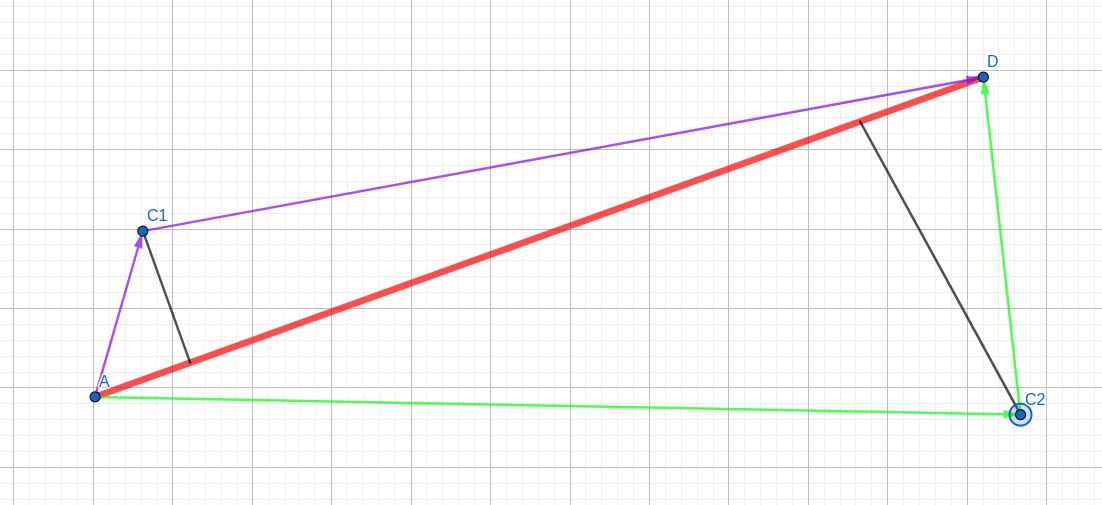
\includegraphics[width=0.7\linewidth]{Afbeeldingen/distances.png}
	\caption{Closest block to arrival and departure point}\label{fig:closest}
\end{figure}

The fact that there are no containers rejected, and the fact that the occupancy
is so low, is noteworthy. This implies that the yard is too big, and the stream
of containers is to little to stress the simulation, even in the slightest way.
This could imply that the stream of containers is to light for this yard.
\begin{table}[h]
	\centering
	\begin{tabular}{|c|c|}
		\hline
		Containers Rejected                         & 0.0        \\ \hline
		CG Rejected                                 & 0.0        \\ \hline
		Normal Rejected                             & 0.0        \\ \hline
		Reefer Rejected                             & 0.0        \\ \hline
		Total Travel Distance                       & 6051683.63 \\ \hline
		AVG Travel Distance Containers              & 380.31     \\ \hline
		AVG daily total Occupancy                   & 0.0366     \\ \hline
		Portion of YB never used                    & 0.7799     \\ \hline
		Portion of YB close to full (at some point) & 0          \\ \hline
		Portion of YB close to full (average)       & 0          \\ \hline
	\end{tabular}
	\caption{FIFO arrival based statistics}
\end{table}
\begin{table}[h]
	\centering
	\begin{tabular}{|c|c|}
		\hline
		Containers Rejected                         & 0.0        \\ \hline
		CG Rejected                                 & 0.0        \\ \hline
		Normal Rejected                             & 0.0        \\ \hline
		Reefer Rejected                             & 0.0        \\ \hline
		Total Travel Distance                       & 7468862.53 \\ \hline
		AVG Travel Distance Containers              & 468.10     \\ \hline
		AVG daily total Occupancy                   & 0.05272    \\ \hline
		Portion of YB never used                    & 0.7799     \\ \hline
		Portion of YB close to full (at some point) & 0          \\ \hline
		Portion of YB close to full (average)       & 0          \\ \hline
	\end{tabular}
	\caption{FIFO departure based statistics}
\end{table}

\subsection{Stressing the system}
\section{Conclusion}
\end{document}